%\date{\copyright\today}
\documentclass[fontsize=12pt,a4paper,draft]{scrartcl}[2003/01/01]

% Das Prozent-Zeichen leitet einen Kommentar ein,
% es hilft ebenso, im Text Leerzeichen zu unterbinden.

% fontsize=12pt  Schriftgroesse in 10, 11 oder 12 Punkt
% a4paper        Papierformat ist hier A4
% landscape      Querformat wird natürlich unterstützt ;-)
% parskip        Absatzabstand anstatt Einzüge
% draft          Der Entwurfsmodus deckt Schwächen auf
% {scrartcl}     Die Dokumentenklasse book, report, article
%                oder fürs deutsche scrbook, scrreprt, scrartcl

\usepackage[ngerman]{babel} % Deutsche Sprachanpassungen
\usepackage[T1]{fontenc}    % Silbentrennung bei Sonderzeichen
\usepackage[utf8]{inputenc} % Direkte Angabe von Umlauten im Dokument.
                            % Wenn Sie an einem Mac sitzen,verwenden
                            % Sie ggf. „macce“ anstatt „utf8“.

\usepackage{textcomp}       % Zusätzliche Symbolzeichen
\usepackage{blindtext}      % Blindtext zum Testen von Textausgaben
\usepackage{graphicx}
%\usepackage{picinpar}
%\usepackage{booktabs}
\usepackage{tabularx}

\title{LastShelter: Survival}
\subtitle{Farming Guide}
\author{\textcopyleft{} anmiwa (Reich449)%
  \thanks{Mit den besten Empfehlungen,
    Wikimedia Foundation Inc.,
    Telefon: +49-0815-4711}}

\date{\today}               % \today setzt das heutige Datum

\begin{document}
\maketitle                  % Titelei erzeugen
\tableofcontents            % Inhaltsverzeichnis anlegen

\listoffigures

\section{Einleitung}
Hier will ich euch eine Anleitung an die Hand geben, wie ihr Farmen für eure Main-Basis anlegen könnt. Ab dem Level 16 wird es sehr schwer die notwendigen Ressourcen durch Plündern von Gegnern zu bekommen. Ein starker Gegner kann einem auch am Ende mehr kosten als nutzen.
Dasselbe gilt für Zombies. Sammeln an den Ressourcen-Stationen ist sehr langwierig und bindet die APC für das Sammeln. Kurz um ihr braucht früher oder später Farmen um voran zu kommen.

Top Spieler mit Level 20 und höher haben zum Teil mehr als 30 Farmen! Ich denke aber für den Anfang sind 3 bis 4 ausreichend.

Da man viel Zeit bräuchte wenn man jede Farm täglich bewirtschaften müsste, ist das Ziel Farmen zu bauen, die maximal einmal pro Woche kurz bearbeitet werden. Das könnte Donnerstag oder Sonntag sein, da hier der Helden Event läuft, der viele Ressourcen für die Farm bringen kann. Siehe Helden-Event.

\begin{table}[h!]
  \centering
    \caption[Ertrag]{Täglicher Ertrag einer fertigen Farm}
    \begin{tabular}{rl}
%      \hline
      Nahrung & 1.617 k \\
      Wasser & 1.944 k \\
      Öl & 1.422 k \\
      Strom & 213 k \\
      Holz & 1.092 k \\
      Eisen & 657 k \\
      Geld & 705 k \\
%\hline\hline
%      \hline
    \end{tabular}
\end{table}

\section{Farm anlegen}
Eine Farm wird angelegt indem man ein neues Spiel startet. Dies kannst du unter Einstellungen/Konto machen.
Jetzt musst du die Einführung ganz normal durchspielen. Bis einschließlich Level 5 hast du einen Schutzschirm,
also gehe nicht auf Level 6 bevor du nicht in unserer Allianz bist und wir dich in unseren Hive transportiert haben.

Deine Farm ist in einem zufälligen Reich (Staat). Du musst also in unseren umziehen. Dazu gehst du auf die Weltkarte.
Unten in der Mitte findest du ein Feld mit den aktuellen Koordinaten. Da klickst du drauf. Jetzt öffnet sich ein 
Fenster (Koordinaten eingeben) in dem du das Reich 449 eintragen musst. X und Y sind erst mal egal.
Wenn du dann im Staat \#449 bist, klickst du in einem freien Bereich, um die Optionen zu sehen. Normalerweise kommt Rechts ein
Button „Staat wechseln“, den wählst du an und bestätigst.
Jetzt sollte deine Basis irgendwo in unserem Staat sein. Damit kannst du dich jetzt für unsere Farm Allianz bewerben.
Du hast auch nur 14 Tage Zeit um den Staat zu wechseln.
Du kannst nach unser Allianz suchen oder auf eine Basis der Allianz klicken [(PaT) daWahnsinn (X:951, Y:411)] oder mich per PM anschreiben,
damit wir dich einladen können.
Wichtig! Der Allianz Teleport funktioniert nur einmal! Danach kostet er 2000 Diamanten! Also am besten gar nicht erst in eine
andere Allianz eintreten.




\begin{figure}[htbp] 
%begin{figure}
  \centering
     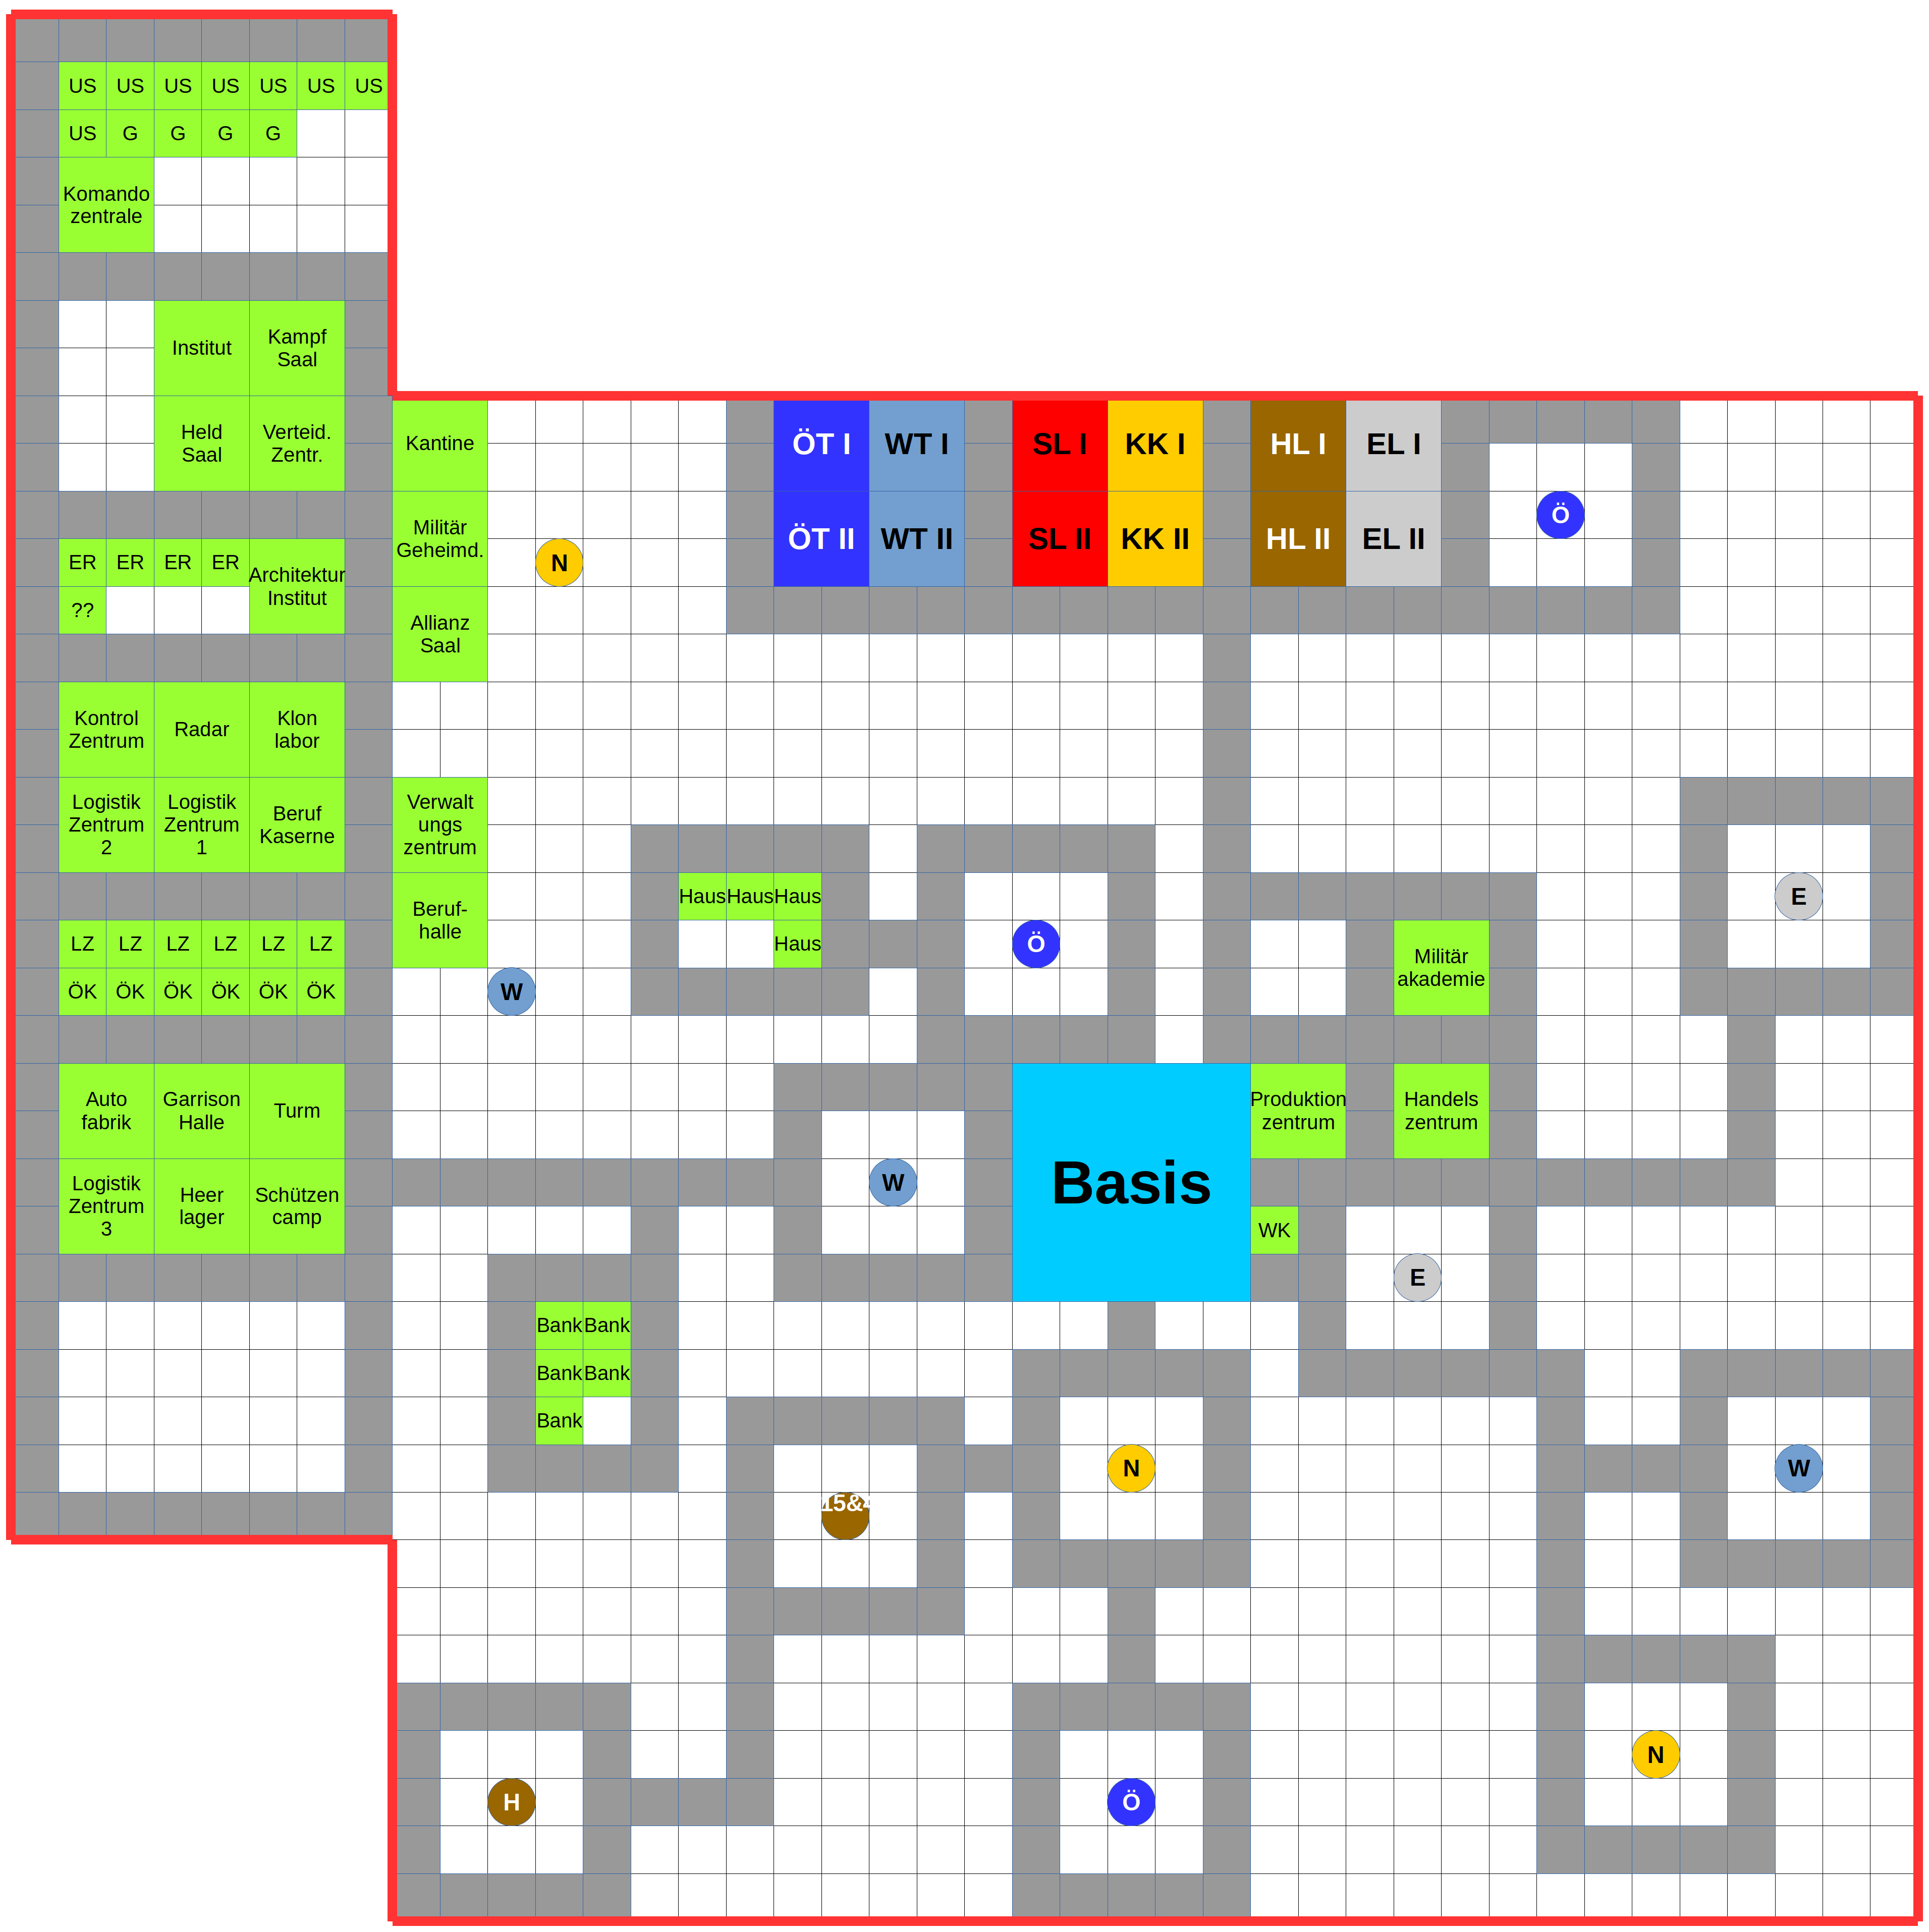
\includegraphics[width=0.7\textwidth]{map.pdf}
%     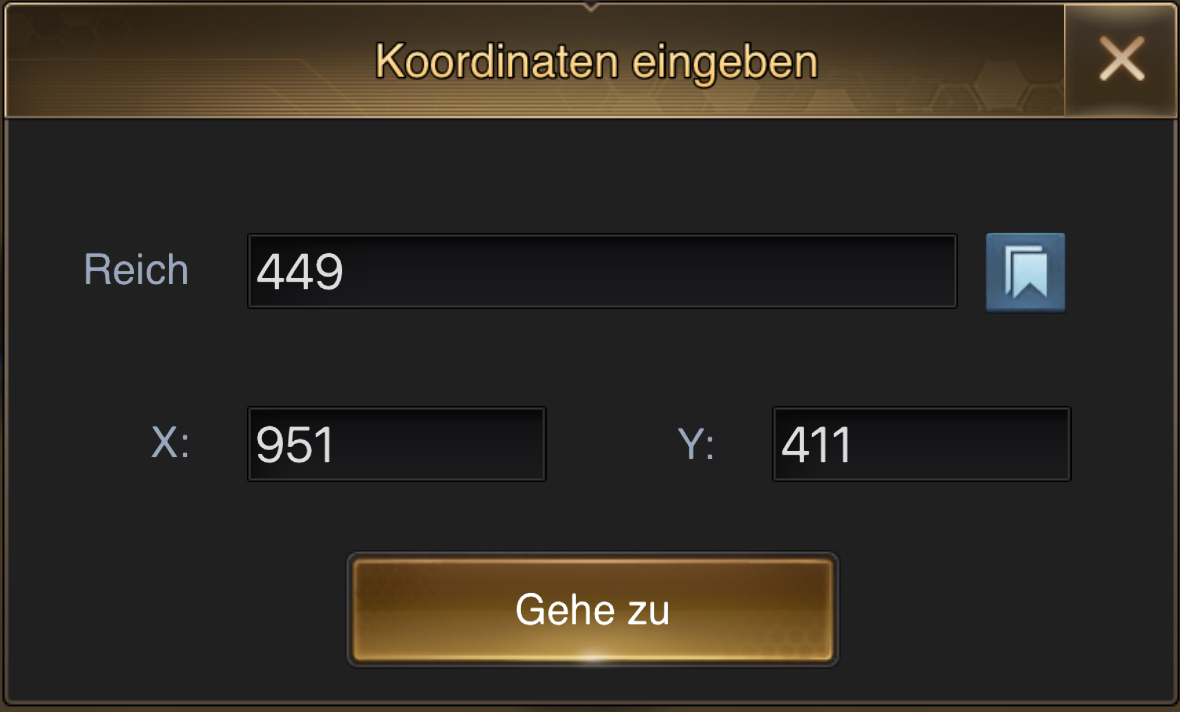
\includegraphics{IMG_E0004.JPG}
  \caption{Erstes Bild}
  \label{fig:Bild1}
\end{figure}

\section*{Zweiter Abschnitt, die Sache mit dem „*“}
Abschnitte werden normalerweise automatisch durchgehend nummeriert, das Setzen eines Sterns -- wie hier in \verb|\section*{}| -- verhindert aber das Auf"|führen der Sektion im Inhaltsverzeichnis und die entsprechende
Nummerierung. So fällt hier im Beispiel der zweite Abschnitt gänzlich unter den Tisch.

\subsection[Die Subsection als Unterabschnitt]{Erster Unterabschnitt}
Unterabschnitte dienen zur weiteren Untergliederung von Abschnitten in einzelne, logische Einheiten. Sie können aber auch als
erklärender Text oder weiter hergeholte Einschübe dienen.

\subsubsection{Empfohlene Gebäude Level}
%Ein demonstrativer Unter-Unterabschnitt \label{Unter-Unterabschnitt}.
%Im Folgenden wird auf diese Textstelle namens Unter-Unterabschnitt~\ref{Unter-Unterabschnitt} verwiesen, die sich hier auf der Seite~\pageref{Unter-Unterabschnitt} befindet.
Nachfolgend eine Liste der benötigten Gebäude und der jeweiligen Level.

\begin{tabularx}{0.9\textwidth}{lccX}
  Gebäude & Level & Straße & Bemerkung \\
  \hline
  Basis & 15 & ja & Nicht höher als 15, da sonst die Punkte für die dritte Kiste bei den Events stak ansteigen. \\
  Windkraftwerk & 15 & ja & Genügt knapp um die Basis mit Strom zu versorgen. \\
  Handelszentrum & 15 & ja & Hier wird Wasser und Strom verkauft. \\
  Militärakademie & 15 & ja & Um die gesammelten Helden in Medallien umzutauschen für die Events. \\
  Institut & 8 & nein & Wird benötigt um Stadtentwicklung auf MAX zu bringen. \\
  Farm & 15 & ja & Nahrung zum plündern. \\
  Sägewerk & 15 & ja & Holz zum plündern. \\
  Klärwerk & 15 & ja & Wasser zum verkaufen. \\
  Ölquelle & 15 & ja & Öl zum plündern. \\
  Eisenmine & 15 & ja & Eisen zum plündern. \\
  Wohnhaus & 15 & ja & Bevölkerung für die Bank-Effizienz. \\
  Bank & 15 & ja & Geld zum plündern. \\
  Lager & 15 & ja & Alle Lager I auf Level 10, damit man Lager II bekommt. \\
  Lager II & 3 & ja & Die Kosten für höhere Level lohnen sich meist nicht. Wenn man regelmäßig seine Farm plündert, sollten 6M Lagerkapazität genügen. \\
  Schützencamp & 13 & nein & Wird benötigt um Basis auf Level 14 upgraden zu können. \\
  Unterschlupf & 8 & nein & ???Wird benötigt um Basis auf Level 9 upgraden zu können. \\
  Lazarett & 9 & nein & ???Wird benötigt um Basis auf Level 10 upgraden zu können. \\
  Produktion Ztr. & 15 & ja & Wenn man Bauer ist, kann hier täglich viele Resourcen bekommen. Allerdings müßte man sich dazu täglich einloggen.\\
  Kantine & 14 & nein & Wird benötigt um Basis auf Level 15 upgraden zu können. \\
  Held Saal & 15 & nein & Wird benötigt um Militärakademie auf Level 15 upgraden zu können. \\
  Öl-Kraftwerk & 9 & nein & Wird benötigt um Stromspeicher auf Level 10 upgraden zu können. \\
  Verteidigungzentrum & x & nein & Hier sollte man ein Level wählen, um mit dem APC des Main 3 mal plündern zu können. \\
  Restliche Gebäude & 1 & nein & Wird nicht benötigt und verbraucht sonst Resourcen. \\
\end{tabularx}

  
%\piccaption{Bildunterschrift} 
%\parpic[r]{
\includegraphics [width=3cm,height=3cm]{TUX.png}}

\subsection[Eine Subsection]{Eine weitere Subsection}
Der Stern oben hat verhindert, dass hier mit 2.2 fortgefahren wird.

\paragraph[Label wird nicht aufgeführt]{%
  Paragraphen tragen keine Label}

Ein Absatz, meist für die klare Aufteilung von Gedankengängen verwendet.

Wie zu sehen, kann ein Absatz auch mehrere Text-Absätze enthalten. Überflüssige Leerzeilen und Leerzeichen werden von \LaTeX{} automatisch heraus gefiltert.

\subparagraph[Ein Subparagraph: Label wird nicht aufgeführt]{Ein Unter-Paragraph}

Diese Schachtelung kann man mit Unter-Paragraphen noch eine Stufe weiter treiben \ldots{}
%
Wir begnügen uns aber mit dem Hinweis auf Unter\-Unterabschnitt~\ref{Unter-Unterabschnitt}.

\section[Aufzählungen]{Aufzählungen und Nummerierungen}
Dieser Abschnitt wird im folgenden beschrieben und kann dann 
hier eingefügt werden.

\section{Mehrere (Farm-) Konten erstellen}

Man kann in LastShelter mehrere Konten mit derselben E-Mail anlegen. Dazu müssen nur Punkte in der E-Mail an beliebiger Stelle vor dem @ eingefügt werden.
Ist deine E-Mail z. B. max.mustermann@gmail.com dann sind gültige Kombinationen: 
\begin{itemize}
  \item m.ax.mustermann@gmail.com
  \item max.m.ustermann@gmail.com
  \item max.muster.mann@gmail.com
\end{itemize}	

Du bekommst immer eine Mail auf deine richtige Addresse, welche du dann bestätigen musst.
So lassen sich beliebig viele Konten mit derselben Adresse erstellen. Das Passwort sollte der Einfachheit halber immer dasselbe sein, muss aber nicht. (Aufschreiben!)


\section{Items}

\begin{description}
  \item[Nahrung:] Wird gefarmt und steht zum Plündern bereit.
  \item[Wasser:] Dient nur zum Verkauf über das Handelszentrum (Hubschrauber)
  \item[Öl:] Wird gefarmt und steht zum plündern bereit.
  \item[Strom:] Wird dringend benötigt, um alles am Laufen zu halten. Die geringe Unterproduktion des Windrades muss durch wöchentliches auffüllen eines Ölkraftwerkes ausgeglichen werden.
  \item[Holz:] Wird gefarmt und steht zum Plündern bereit.
  \item[Eisen:] Wird gefarmt und steht zum Plündern bereit.
  \item[Geld:] Wird gefarmt und steht zum Plündern bereit.
  \item[Bevölkerung:] Wird für Geld Produktion benötigt. Ohne tägliches Auffüllen der Kantine sinkt die Bevölkerung auf 66\%, was für Händler ausreichen ist.
  \item[Diamanten:] Werden in großen Mengen durch Heldentausch Trick gewonnen
  \item[Truppen:] Diese werden nicht benötigt und würden nur Nahrung verschwenden
\end{description}



\section{Tips für Farmen}
\begin{itemize}
  \item Farmen nur bis maximal Level 15 hochrüsten, da sonst die täglichen Events für die dritte Kiste zu teuer wird.
  \item Händler bekommen zwar weniger Ressourcen, aber 50\% mehr Geld. Wenn man sich nicht täglich um die Farm kümmern möchte, lieber Händler nehmen. Sonst natürlich Bauer.
  \item Windkraftwerk immer auf höchstem Level, um möglichst lange ohne Interaktion (Öl auffüllen) auszukommen.
  \item Alles was man nicht braucht von der Straße entfernen. Spart Strom.
  \item Wenn man die maximale Bevölkerungszahl erreicht hat, kann man die Kantine leer werden lassen und die Straße entfernen. Die Bevölkerung sinkt dann auf 66\% wie auch die Geldproduktion. Durch die 50\% plus des Händlers, hat man wieder 100\%.
  \item Die Lager II bis maximal Level 3, da diese dann extrem teuer werden. 7M sollten genügen.
\end{itemize}	


\end{document}